%%%%%%%%%%%%%%%%%%%%%%%%%%%%%%%%%%%%%%%%%
% Journal Article
% LaTeX Template
% Version 1.4 (15/5/16)
%
% This template has been downloaded from:
% http://www.LaTeXTemplates.com
%
% Original author:
% Frits Wenneker (http://www.howtotex.com) with extensive modifications by
% Vel (vel@LaTeXTemplates.com)
%
% License:
% CC BY-NC-SA 3.0 (http://creativecommons.org/licenses/by-nc-sa/3.0/)
%
%%%%%%%%%%%%%%%%%%%%%%%%%%%%%%%%%%%%%%%%%

%----------------------------------------------------------------------------------------
%	PACKAGES AND OTHER DOCUMENT CONFIGURATIONS
%----------------------------------------------------------------------------------------

\documentclass[twoside,twocolumn]{article}

\usepackage{blindtext} % Package to generate dummy text throughout this template 

\usepackage[sc]{mathpazo} % Use the Palatino font
\usepackage[T1]{fontenc} % Use 8-bit encoding that has 256 glyphs
\linespread{1.05} % Line spacing - Palatino needs more space between lines
\usepackage{microtype} % Slightly tweak font spacing for aesthetics

\usepackage[english]{babel} % Language hyphenation and typographical rules

\usepackage[hmarginratio=1:1,top=32mm,columnsep=20pt]{geometry} % Document margins
\usepackage[hang, small,labelfont=bf,up,textfont=it,up]{caption} % Custom captions under/above floats in tables or figures
\usepackage{booktabs} % Horizontal rules in tables

\usepackage{lettrine} % The lettrine is the first enlarged letter at the beginning of the text

\usepackage{enumitem} % Customized lists
\setlist[itemize]{noitemsep} % Make itemize lists more compact

\usepackage{abstract} % Allows abstract customization
\renewcommand{\abstractnamefont}{\normalfont\bfseries} % Set the "Abstract" text to bold
\renewcommand{\abstracttextfont}{\normalfont\small\itshape} % Set the abstract itself to small italic text

\usepackage{titlesec} % Allows customization of titles
\renewcommand\thesection{\Roman{section}} % Roman numerals for the sections
\renewcommand\thesubsection{\Roman{section} \Alph{subsection}} % roman numerals for subsections
\titleformat{\section}[block]{\large\scshape\centering}{\thesection.}{1em}{} % Change the look of the section titles
\titleformat{\subsection}[block]{\large}{\thesubsection.}{1em}{} % Change the look of the section titles

\usepackage{fancyhdr} % Headers and footers
\pagestyle{fancy} % All pages have headers and footers
\fancyhead{} % Blank out the default header
\fancyfoot{} % Blank out the default footer
\fancyhead[C]{State of Art of Artificial Neurals Networks Compression} % Custom header text
\fancyfoot[RO,LE]{\thepage} % Custom footer text

\usepackage{titling} % Customizing the title section

\usepackage{hyperref} % For hyperlinks in the PDF

\usepackage{amsmath,array}
\newcommand*{\vertbar}{\rule[-1ex]{0.5pt}{2.5ex}}
\newcommand*{\horzbar}{\rule[.5ex]{2.5ex}{0.5pt}}

\usepackage{graphicx}
\graphicspath{ {./images/} }
%----------------------------------------------------------------------------------------
%	TITLE SECTION
%----------------------------------------------------------------------------------------

\setlength{\droptitle}{-4\baselineskip} % Move the title up

\pretitle{\begin{center}\Huge\bfseries} % Article title formatting
\posttitle{\end{center}} % Article title closing formatting
\title{State of Art in Artificial Neurals Networks Compression} % Article title
\author{%
\textsc{Pierre Gabin FODOP GUMETE} \\[1ex] % Your name
\normalsize ENSTA Bretagne \\ % Your institution
\normalsize \href{mailto:pierre.fodop@ensta-bretagne.org}{pierre.fodop@ensta-bretagne.org} % Your email address
%\and % Uncomment if 2 authors are required, duplicate these 4 lines if more
%\textsc{Jane Smith}\thanks{Corresponding author} \\[1ex] % Second author's name
%\normalsize University of Utah \\ % Second author's institution
%\normalsize \href{mailto:jane@smith.com}{jane@smith.com} % Second author's email address
}
\date{\today} % Leave empty to omit a date
\renewcommand{\maketitlehookd}{%
\begin{abstract}
  In the last twenty years, we have seen an exponential increase in the computing power of personal computers, in addition 
  to the explosion of cloud services and the increase in the number of server farms for data storage. One of the 
  consequences of this increase was to make a certain amount of data available to as many people as possible, but also 
  the explosion of Neural Networking methods with the objective of use this data. They have been applied to a large 
  number of problems, in particular in image processing, sound processing, natural language processing (...) Areas in 
  which they currently constitute the state of the art. On the other hand, we have also had a significant advance in the 
  Internet of Things, which creates the need for neural networks adapted to powerful objects. The objective of this article 
  is to present the different methods to compress neural networks and thus store networks in a smaller space, but also to 
  accelerate calculations with them.
\end{abstract}
}

%----------------------------------------------------------------------------------------

\begin{document}

% Print the title
\maketitle

%----------------------------------------------------------------------------------------
%	ARTICLE CONTENTS
%----------------------------------------------------------------------------------------

\section{Introduction}
The history of neural networks begins with Warren S. McCulloch and Walter Pitts of MIT researchers who presented in 1943 an
article on the realization of neural functions by electrical functions and logic gates.\cite{warren1}.
Their approach is linked to a perception of neuronal functions as {\bf\textit{all or nothing}} functions. 
This advance will be completed later by the definition of the perceptron\cite{RosenBlatt1} and the discovery of the gradient 
back-propagation algorithm\cite{Rumelhart1}.

\begin{figure}[h]
\centering
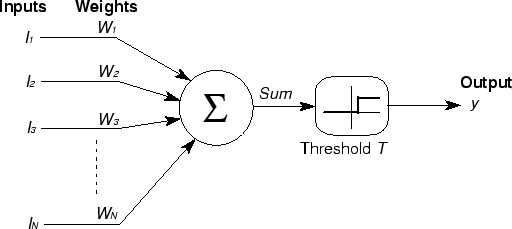
\includegraphics[width=70mm]{CulochNeurone.png}
\caption{McCulloch and Pitts Computational Model}
\label{SimpleNeuron}
\end{figure}

With the \textit{winter of arrtificial l'Intelligence} which will begin at the end of the 1960s, advances in the field of 
artificial intelligence will be slower.Also because of a reduction in both public and private investments in this field. 
Although slowed down, it was during this period that the first large-scale implementations of expert systems designed in 
1950 were designed. Here, most intelligent systems work with a so-called \textit{Knowlege Based} base. We have the development 
of the bases of methods such as Inductive Logic Programming (ILP)\cite{Muggleton1}\cite{Ehud1}. Which will later be compiled 
by S.H. Muggleton in his founding article "Inductive Logic Programming"\cite{Muggleton2}.

Finally, in the 1990s, there was a comeback of artificial intelligence with new methods and with the increase in computing power; 
this with the advent of the first Pentium processors by Intel, a generalization of supercomputers and finally the advent of the 
Internet which will allow an unprecedented exchange of knowledge. This evolution will reach a first major palliative in 2012 with 
the application of neural networks to the ImageNet image classification challenge which will make it possible to reduce the lowest 
rate of classification error from 25 \% to 16 \% thanks to the AlexNet network\cite{Rajat1}. 

Since then, neural networks have been applied to an increasing number of problems. especially in Computer Vision\cite{MadhusmitaSahu}
\cite{Sornaminproceedings}, en Natural language processing\cite{jing2019survey}, in signal analysis\cite{MohamedIbn1}\cite{XiaofanLi1} 
an other. \cite{POZNYAK2019250} With better results than the methods that were used until then. This has created the need for neural 
networks suitable for a certain number of supports. In particular media from the Internet of Things.

The objective of this document is to make a tour of the methods allowing to compress neural networks and to apply them in a certain number 
of objects, to do this, we will start by making a presentation of the different existing neural network architectures. , then, we will 
explore the methods of pruning, sparse representation in particular quantified, knowledge distillation and finally, we will see the future methods

%------------------------------------------------

\section{Types of Neurals Networks}

\subsection{The Perceptron}

It is the simplest expression of a neural network, it consists of a single formal neuron\cite{warren1}.

\begin{figure}[h]
  \centering
  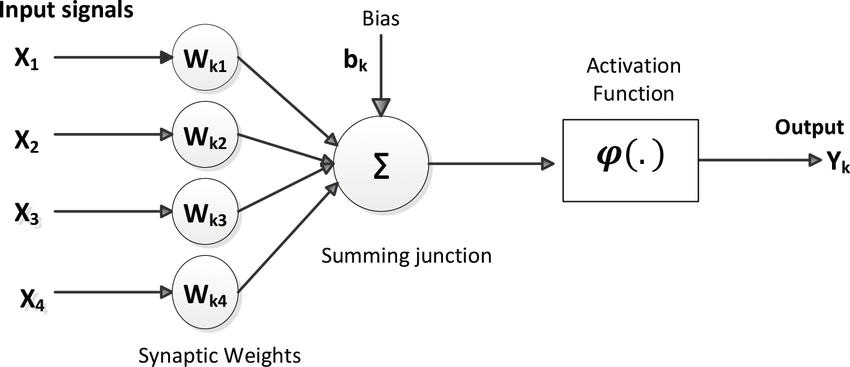
\includegraphics[width=70mm]{McCulloch-Pitts-computational-model-of-a-neuron.png}
  \caption{Simple Perceptron }
  \label{PerceptronMathematique}
\end{figure}

The neuron took as input a vector of values $x$, multiply then with a weigth vector $w$ finally thanks to the activation function returns 
the exit to us.
\[
y = \varphi(
\left[
  \begin{array}{ccc}
    w_{1}\\
    w_{2}\\
    w_{3}\\
    w_{4}\\  
  \end{array}
\right]*
\begin{bmatrix}
           x_{1} \\
           x_{2} \\
           x_{3} \\
           x_{4}
         \end{bmatrix}
+ b)\]
The activation function $\varphi()$ must meet a number of conditions.
\begin{itemize}
  \item \textbf{Identity in zero} si $f(x) = 0$ alors $x = 0$ \cite{Sussillo2014RandomWI} These functions allow you to make learning more 
  quickly.
  \item \textbf{Monotonic value derivative}\cite{WU20093432} for a better generalization capacity and an ease of application of the convex 
  optimization methods.
  \item \textbf{Everywhere Differentiable}\cite{Rumelhart1} allowing the application of gradient descent.
\end{itemize}

To update the weights $ w $ of our perceptron, we will use the gradient descent algorithm. The latter allows, from a chosen error function, 
to update these weights.Let $ F (x) $ be a defined and differentiable function close to the local minimum point $ a $. The objective is to 
estimate the value of a; we will define a learning coefficient $ \ lambda $. We will therefore define the following sequence with an 
initialization at $ a_0 $.

\[\left\{
  \begin{array}{rcr}
    a_{0} & =  a_0 \\
    a_{n+1} & = & a_{n} - \lambda. \Delta F(a_n)\\
  \end{array}
\right.\]

For a neuron network with the sigmoid function as an activation function and the \textit{cross entropy loss} function as an loss function.

$E(y) = -(y^v.log(y) + (1-y^v).log(1-y))$
\[ \frac{\partial E}{\partial w}
   = \frac{\partial E}{\partial y}
   *\frac{\partial y}{\partial z}
      *\frac{\partial z}{\partial w}\]

\[ \frac{\partial E}{\partial y}
  =  \frac{y^v}{y} - \frac{1-y^v}{1-y}
  = \frac{y^v - y}{y(1 - y)} \]

\[ \frac{\partial y}{\partial z}
  =  y*(1-y) \]

\[ \frac{\partial z}{\partial w}
  =  w^T \]

\[ \frac{\partial E}{\partial w}
  = x*(y^v-y) \]

Where we had 
\[\left\{
  \begin{array}{rcr}
    w_{0} & =  w_0 \\
    w_{n+1} & = & w_{n} - \lambda.(y^v-y).x\\
  \end{array}
\right.\]
The procedure is identical for updating the biases.

At its exit, a neuron makes it possible to classify a class into two classes of values. Those which activate the neurons and those which do 
not activate it; more than one can be used to classify into a larger number of classes. We will then obtain multi-layer perceptrons

\subsection{The Multi-Layer perceptrons}
This is the most basic type of neural network, it is made up of a certain number of layers itself made up of formal neurons.\cite{warren1}. 
The information is thus transmitted from the first layer called the input layer to the last layer called the output, passing through the cache 
layers through the connection between the neurons. In the case where each neuron of a layer is linked to all the neurons of the following 
layer, we speak of fully connected networks.

\begin{figure}[h]
  \centering
  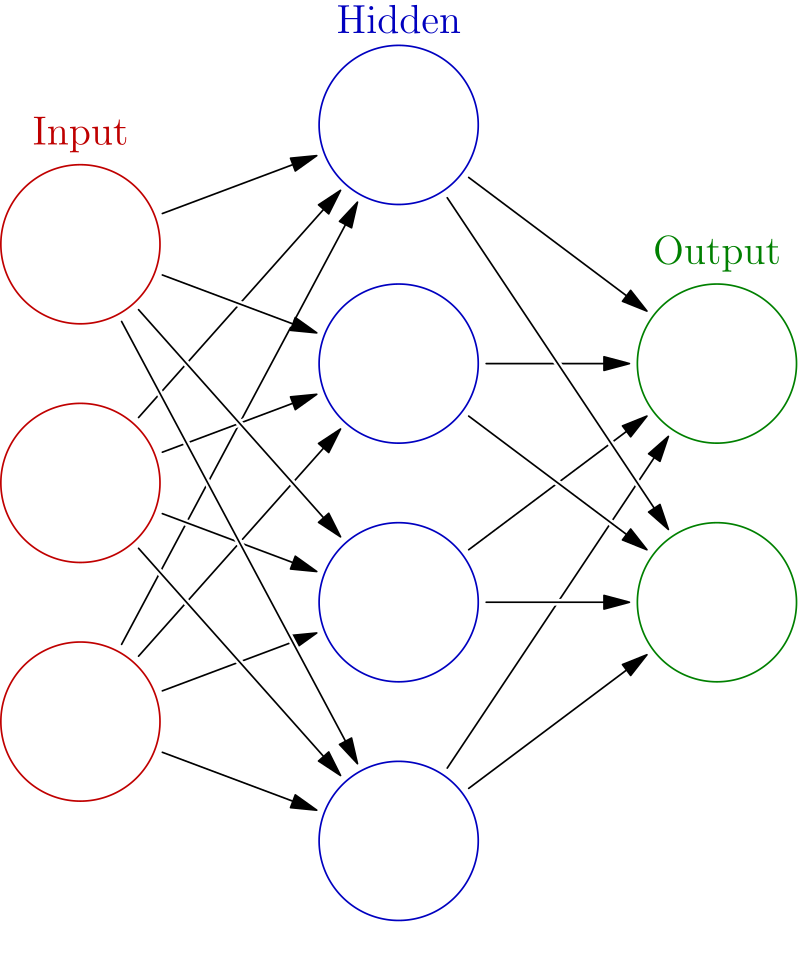
\includegraphics[width=60mm]{Colored_neural_network.png}
  \caption{Multi-Layer perceptrons}
  \label{PerceptronMulticouche}
  \end{figure}
Currently, multi-layered perceptrons, under the best conditions, obtain an error rate of less than 0.35 \%\cite{DeepBig} The mathematical equivalent 
of a network with 784 input 16 caches and 10 output neurons is as follows:

\[
y^1 = \varphi_1(
\left[
  \begin{array}{ccc}
    w_{1}^{1} & ... & w_{1}^{784}\\
    \vdots & \vdots & \vdots\\
    w_{16}^{1} & ... & w_{16}^{784}\\
  \end{array}
\right]*
\begin{bmatrix}
           x_{1} \\
           \vdots \\
           x_{784}
         \end{bmatrix}
+ \begin{bmatrix}
  b_{1} \\
  \vdots \\
  b_{784}
\end{bmatrix}
)\]

\[
y^2 = \varphi_2(
\left[
  \begin{array}{ccc}
    w_{1}^{1} & ... & w_{1}^{16}\\
    \vdots & \vdots & \vdots\\
    w_{10}^{1} & ... & w_{10}^{16}\\  
  \end{array}
\right]*
\begin{bmatrix}
           x_{1} \\
           \vdots \\
           x_{10}
         \end{bmatrix}
+ \begin{bmatrix}
  b_{1} \\
  \vdots \\
  b_{10}
\end{bmatrix}
)\]
To make a probabilistic distribution of the outputs, we can use a certain number of functions, in this case we will use a softmax function.

\[
out = softmax(y^2)
\]
we will therefore have a vector of 10 probabilities, which each signifies if the class represented is the adequate class.


\subsection{Convolutionnals Neurals Networks (CNNs)}
%------------------------------------------------
The greatest flaw of multi-layered perceptron-type networks is their inability to process an image as aggregate information has led to the 
development of Convolutional neural networks.

Filtering for an image is a mathematical operation that allows a matrix called a kernel to do a number of operations on an image. One can 
quote among these last the blurring, the detection of contour. This will be done by convolution of a matrix called nucleus with an our image. 
its mathematical representation is as follows:

\[g(x,y) = w*f(x,y)\]
\[w*f(x,y) = \sum_{dx=-a}^{a} \sum_{dx=-b}^{b} w(dx,dy)f(x+dx,y+dy)\]

In the context of contour detection which is one of the bases of convolutional neural networks, Canny filtering will preferably be used\cite{Canny1}.

\begin{figure}[h]
  \centering
  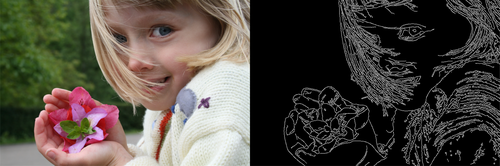
\includegraphics[width=60mm]{canny.png}
  \caption{Canny Filtering}
  \label{CannyOutput}
  \end{figure}

For a convolutional layer, we will apply to our image a certain number of convolutional filters which will allow us to capture as much information 
as possible on the image. We will be able to apply a Pooling on the filtered images obtained to reduce the number of dimensions.

  \begin{figure}[h]
  \centering
  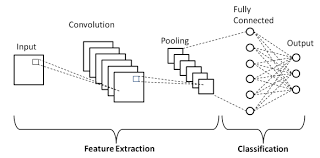
\includegraphics[width=72mm]{convneural.png}
  \caption{Convolutionnal Network}
  \label{ConvNet}
\end{figure}
And at the end of the network, we apply a Multi layer perceptrons network to classify the images. It is also possible to have a fully convolutional network. 

There are many applications of convolutional networks, as much in image processing \cite{Browne1} (VGG16, LeNet, ...), as in natural language processing 
\cite{8666928}, or in audio signal processing \cite{Gama_2019}. Although convolutional neural networks complement perceptron networks, they have the limitation 
of not taking into account temporal values and are quite useful for analyzing sequences such as video sequences.


\subsection{Recurents Neurals Networks}

Recurrent networks, we were created to allow a transfer of information in the cells taking into account the infulence of time.
Here we are talking about a double spatial temporal propagation. This gives the ability to these neurons to intervene in the analysis of phenomena evolving over 
time such as videos, time series ...

Recurrent networks have emerged with the Hopfield \cite{Hopfield} network. The latter introduces memory into the networks allowing information to pass through 
time. They will experience some evolutions until the arrival of another type. Network of neurons, The \textit{Long Short Term Memory} \cite{lstm1}

\begin{figure}[h]
  \centering
  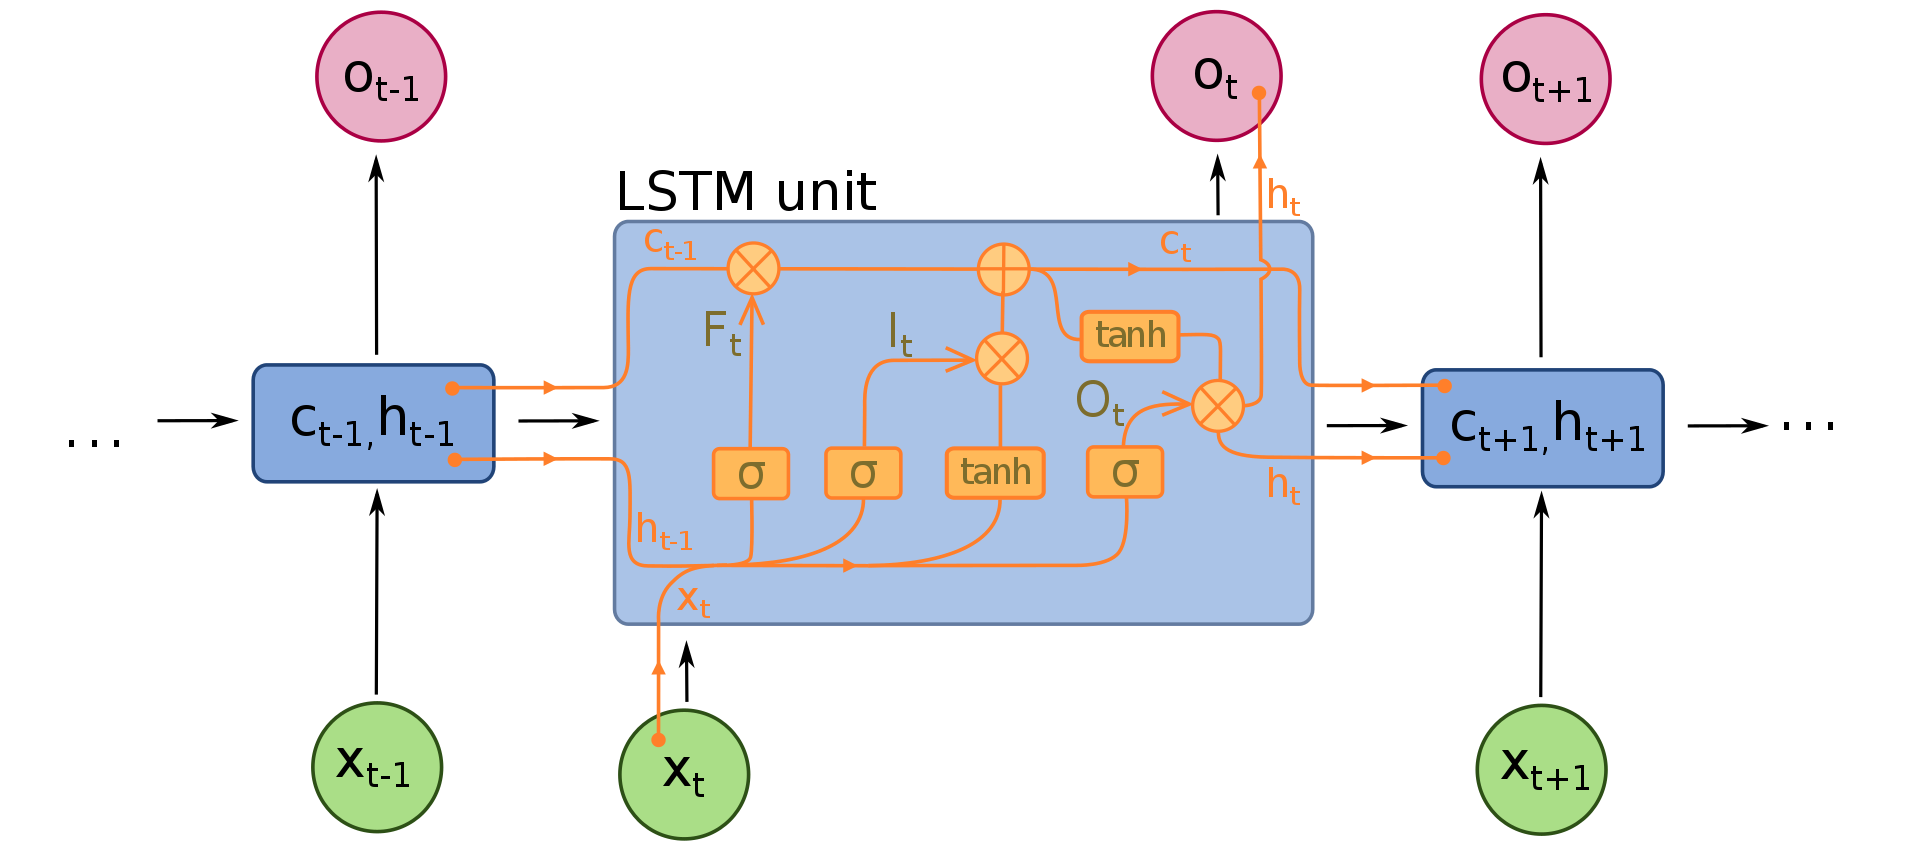
\includegraphics[width=72mm]{Long_Short-Term_Memory.png}
  \caption{LSTM Cell}
  \label{lstm}
\end{figure}

Une celule LSTM prend en entree 3 valeurs valeurs, les sorties de la celule precedente $H_t$ l'etat cache et $C_t$ l'etat de la celule; mais aussi la valeur actuelle d'entree $X_t$. 

la premiere porte que nous verons est porte de l'oublie. la fonction de la porte d'oublie est la suivante:
\[f_t = \sigma(U^fX_t + W^fh_{t-1})\]
Les portes suivantes permettent de calculer l'etat d'entree et l'etat de sortie
\[i_t = \sigma(UX_t + Wh_{t-1})\]
\[O_t = \sigma(U^{\circ}X_t + W^{\circ}h_{t-1})\]
Output Dors
\[g_t = tanh(U^gX_t + W^gh_{t-1})\]
final state of cell
\[c_t = i_tg_t + f_tc_{t-1}\]
Next Hidden state
\[h_t = tanh(c_t)o_t\]

Finally, in 2014, the so-called Gated Recurrent Unit (GRUs)\cite{cho2014learning}. 

\begin{figure}[h]
  \centering
  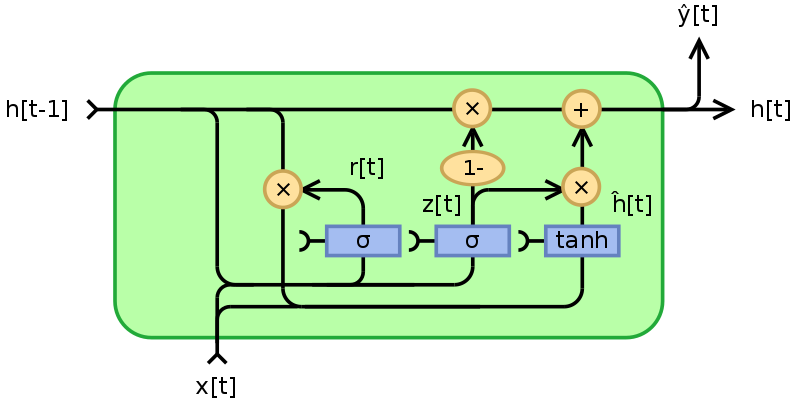
\includegraphics[width=70mm]{GRU.png}
  \caption{GRU Cell}
  \label{GRUs}
\end{figure}

La cellule GRU prend en entre 2 variables et genere deux sorties. Les entrees sont $h_t$ l'etat cache provenant de la precedente cellule 
$x_t$ la valeur actuelle de l'entree ; les sorties sont quant a elles, $y^est$ la valeur de sortie estimee et $h_t$ l'etat cache estime.

On the mathematics point of vue we have:
\[z_t = \sigma_g(W_{z}x_{t} + U_{z}h_{t-1} + b_{z})\]
\[r_t = \sigma_g(W_{r}x_{t} + U_{r}h_{t-1} + b_{r})\]
\[h_{t}^{est} = \phi_h(W_{h}x_{t} + U_{h}(r_t * h_{t-1}) + b_{h})\]
\[h_t = (1 - z_t)*h_{t-1} + z_t*h_{t}^{est}\]
Where $x_t$ is the input vector, $h_t$ the output vector, $z_t$ the update dors vector, $r_t$ reinitialisation vector, $h_t^{est}$ Vecteur candidat d'acivaion.
$W$, $U$ et $b$ sont les marices de parametre. $\sigma_g$ is the sigmoide  fonction and $\phi_h$ est la tangente hyperbolique.

More recently, the GRUs have been modified to give the Minimal Gated Unit networks \cite{heck2017simplified} \cite{zhou2016minimal}. These networks have the advantage 
of having a minimum of input output and logic gate.

\begin{figure}[h]
  \centering
  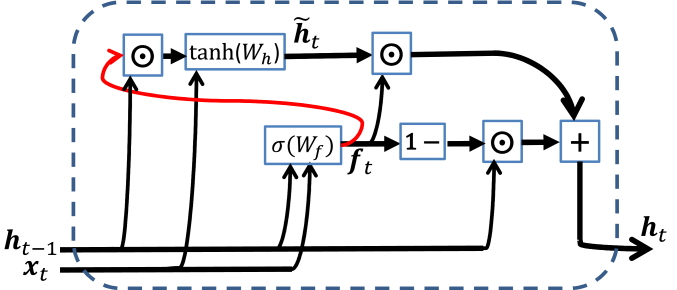
\includegraphics[width=70mm]{MRU.png}
  \caption{MRU Cell}
  \label{MRUs}
\end{figure}

\subsection{Others Networks}
The types of neural networks presented above all have the particularity of being in supervised learning. This kind of network is generally used for classification. 
In this part we will focus on the case of other types of networks whose learning is generally unsupervised.

the first of these networks will be, \emph{Bolztmann Machines}. the origin of these networks is the article by Hinton and Sejnowski of 1983 \cite{Rumelhart2}, they 
are used to have probabilistic distribution estimates of a data set \ cite {Salakhutdinov}. These are generally used in the form of a Bolzmann machine restricted 
to two layers of neurons.

Next we have the \emph{Markov chains}. Here we have a network which based on knowledge of the current state and a set of known probabilities can predict future states. 
They are used on discrete time, or continuous time and discrete state space processes.

Enfin nous classeron un certain nombre de reseaux notemment les auto encodeur (auto-encodeur variationnel, auto encodeur de debruitage), les Reseaux generatifs adversariaux (...) dans la cathegorie des reseaux composees
en cela qu'il sont issue de la composition d'un certain nombre de couche de neuronne issue des reseaux mentionne plus haut.

\section{Why the compression of neural networks}%----------
The origin of connected objects dates back to 1994 when the start-up Violet launched the concept of the DAL wifi connected lamp. And since then their number has 
not stopped growing, their use too. On the other hand, the number of computer tools has also increased considerably, with the invention of smartphones, tablets and others..

These connected objects have in common that they have neither great computing power nor large storage space. This situation removes them from the possibility of 
aplication of neural networks which when we needed significant computing power and also large storage space.

\begin{table}[!h]  
\begin{tabular}{|l|c|r|}
    \hline
    DNN & Size(MB) & Temps(Milion) \\
    \hline
    AlexNet & 200 & 720 \\
    VGG-16 & 550 & 15 300 \\
    GoogLeNet & 50 & 1550 \\
  ResNet & 170 & 11 300 \\
  \hline
\end{tabular}
\caption{Les Poids et temps de calcul de differents reseaux}
\end{table}

To make these objects smarter, it is therefore important for us to be able to develop suitable neural networks. To do this, a number of ways and methods have been 
developed. Among the methods which tackle to reduce the weight of the networks one has, The pruning, the quantification, the distillation of knowledge. Other approaches 
aim at a distribution of calclus between several objects such as federe learning. Here we will explore in depth the approaches that attempt to reduce the size of networks 
and we will make an introduction to federe learning. Finally, as far as possible, we will present the results that we had by modeling the methods.

\section{Le Pruning} %-------------------------------

\subsection{C'est quoi le Pruning}
One of the first ideas for reducing the size of memory networks is to remove unnecessary connections between neurons. Indeed, during the training of neural networks and 
their use, there are potentially connections that have never been activated, their suppression therefore saves storage space.

Pruning is the method of reducing the size of neural networks which consists in removing weights below a certain threshold.

\begin{figure}[h]
  \centering
  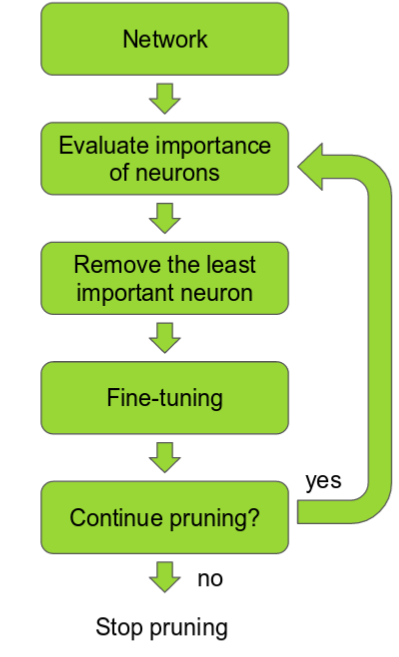
\includegraphics[width=40mm]{pruning_steps.png}
  \caption{Steps of Pruning}
  \label{Pruning_step}
\end{figure}

\begin{figure}[h]
  \centering
  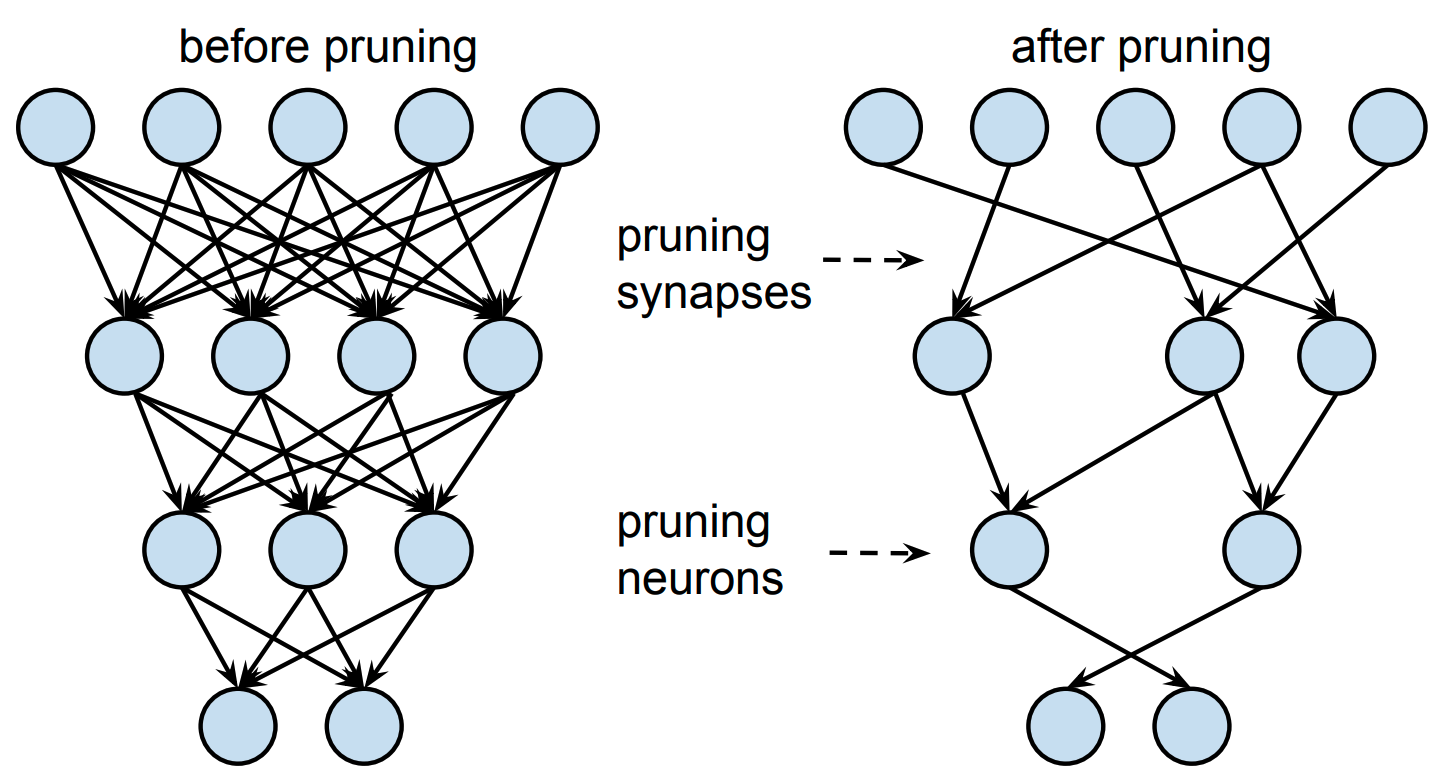
\includegraphics[width=70mm]{pruning.png}
  \caption{Pruning}
  \label{pruning of perceptron Multi-Layer perceptron}
\end{figure}
Research in this area is directed towards solving the resulting compression / efficiency problem.

In the following section, we will present the state of the art of the pruning method by focusing on some publications that we have selected.

\subsection{State of the art of the Pruning method}

The first major publication which laid the groundwork for the application of the pruning method dates back to 1991 \ cite {SYKung}. the main idea of the latter is to 
use the mean square error associated with the Forbenius norm for

\subsection{Le futur du Pruning}
\subsection{Presentation de mes resultats}

\section{Quantification}%---------------------
\subsection{Quantification}
\subsection{Binarization}

\section{Distillation de connaissance} %--------------


\section{Autres Methodes}%-----------


\section{Conclusion}%---------

%----------------------------------------------------------------------------------------
%	REFERENCE LIST
%----------------------------------------------------------------------------------------

\bibliographystyle{plain}
\bibliography{reference} 

%----------------------------------------------------------------------------------------

\end{document}
